\chapter{Implementacja}

W niniejszym rozdziale zostanie przedstawiona koncepcja realizacji projektu wraz z opisem używanych
technologii.

\section{Opis projektu}

Projekt wykorzystuje zarówno architekturę klient-serwer jak i architekturę P2P.

Na projekt składają się dwie części, serwer oraz aplikacja graficzna (klient).

Serwer pełni dwie funkcje:

\begin{itemize}
	\item odkrywanie - tj. pozwala połączonym klientom ogłosić swoją dostępność oraz wysyła klientom
	      listę innych połączonych klientów
	\item sygnalizacja - aby utworzyć połączenie peer-to-peer pomiędzy klientami, niezbędna jest
	      między nimi wymiana informacji przez jakiś inny kanał. W tym celu serwer pośredniczy w wymianie
	      wiadomości pomiędzy klientami.
\end{itemize}

Celem klienta jest połączenie z serwerem, a następnie jednoczesne nasłuchwanie na wiadomości od
serwera oraz reagowanie na zdarzenia pochodzące od użytkownika.

Poszczególne połączenia nawiązywane przez klientów realizowane są w architekturze P2P.

\begin{figure}[H]
	\centering
	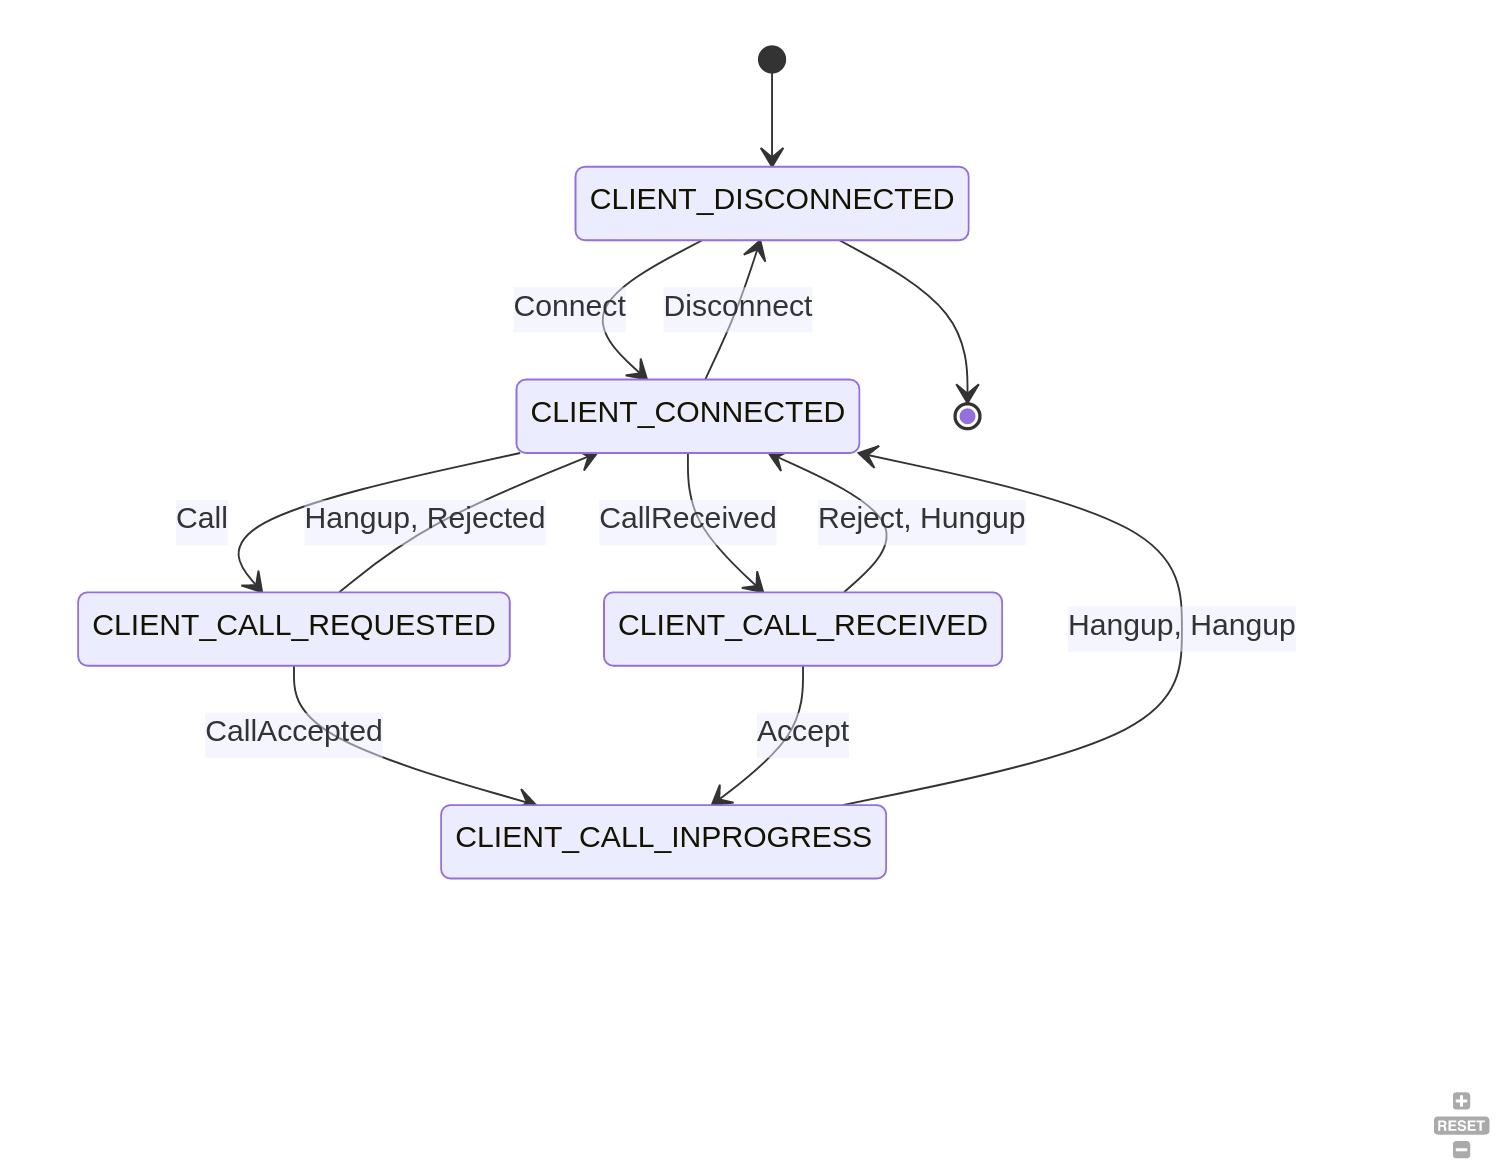
\includegraphics[width=.8\textwidth]{img/rozdzial3/state-diagram-2}
	\caption{Diagram stanów klienta}
\end{figure}

Zarówno wiadomości od klienta (rozpoczęcie połączenia, rozłączenie się) jak i od serwera (pojawił
się nowy użytkownik, otrzymano połączenie) mogą pojawić się w każdym momencie, więc model
komunikacji request/response będzie niewystarczający. Potrzebny jest model komunikacji gdzie każda
ze stron nasłuchuje na przychodzące zdarzenia od drugiej strony połączenia.

\subsection{Serwer}

Do komunikacji wykorzystywane są protokoły TCP i WebSockets. TCP zapewnia gwarancję poprawności
odebranych danych i ich odpowiedniej kolejności, zamienia strumień pakietów na łańcuch bajtów
przychodzący w kolejności. Protokół Websockets zapewnia framing, czyli zamienia łańcuch bajtów na
strumień wiadomości które mogą mieć różną wielkość i zawierać dane tekstowe lub binarne. Protokół
aplikacji wykorzystuje tylko dane tekstowe.

\subsubsection{Protokół aplikacji}

Rodzaje komunikatów możliwych do wysłania przez klient lub serwer są zebrane w odpowiedni typ
wyliczeniowy a następnie w wiadomości tekstowej Websockets wysyłana jest ich serializacja w formacie
JSON.

\begin{minted}{rust}
use serde::{Deserialize, Serialize};

#[derive(Serialize, Deserialize, Debug, Clone)]
#[serde(rename_all = "lowercase")]
pub enum Message {
    Connect(ConnectMessage),
    ConnectResponse(ConnectResponse),
    UserList(UserList),
    Webrtc(WebrtcMsg),
    Call(CallMessage),
    CallReceived(CallReceivedMessage),
    CallHangup,
    CallResponse(CallResponseMessage),
}
\end{minted}

Implementacja serwera wykorzystuje dwie techniki komunikacji wieloprocesowej:

\begin{itemize}
	\item synchronizacja dostępu do dzielonych danych
	\item przekazywanie wiadomości
\end{itemize}

\section{Klient}

Aplikacja okienkowa składa się z czterech konkurentnie wykonujących się zadań:

\begin{enumerate}
	\item Zadanie GUI, rysuje okienko oraz emituje zdarzenia GUI
	\item Zadanie połączenia z serwerem, nasłuchuje wiadomości wysłane przez serwer oraz emituje
	      zdarzenia sieciowe
	\item Zadanie połączenia, prowadzi proces sygnalizacji i negocjacji WebRTC, a następnie prowadzi
	      połączenie: prezentuje strumienie audio-wideo użytkownikowi oraz wysyła strumienie wideo i
	      audio drugiej stronie połączenia. Działa od rozpoczęcia połączenia do jego zakończenia.
\end{enumerate}

Rdzeń aplikacji odpowiedzialny jest za odbieranie zdarzeń od zadań i reagowanie na nie wysyłając
komendy do innych zadań. Np. odbieranie zdarzenia kliknięcia w przycisk rozpoczęcia połączenia
obok użytkownika X powoduje wysłanie komendy "zadzwoń do użytkownika X" do zadania połączenia.
Podobnie gdy zadanie połączenia odbierze od serwera wiadomość \verb|UserList|, rdzeń odbiera to
zdarzenie i wysyła komendę do zadania GUI by zaktualizowało listę dostępnych użytkowników.

Wyjątkiem jest zadanie GStreamer które komunikuje się bezpośrednio z zadaniem połączenia. Powody
takiej decyzji są dwa:

\begin{itemize}
	\item Zadanie GStreamer wysyła i odbiera dużą ilość danych które nie mają żadnego efektu w GUI,
	      więc bezpośrednie połączenie sprawia że rdzeń nie musi być ich świadom
	\item Dopóki trwa rozmowa, użytkownik nie może rozpoczynać ani odbierać żadnych nowych rozmów
\end{itemize}

\subsection{Zadanie GUI}

GUI emituje następujące zdarzenia:

\begin{minted}{rust}
#[derive(Debug)]
pub enum GuiEvent {
    CallStart(u32),
    CallAccepted(VideoPreference),
    CallRejected,
    NameEntered(String),
}
\end{minted}

\subsection{Zadanie połączenia}

Zadanie połączenia emituje następujące zdarzenia:

\begin{minted}{rust}
#[derive(Debug)]
pub enum NetworkEvent {
    UserlistReceived(Vec<(u32, String)>),
    CallReceived(String),
}
\end{minted}

\subsection{Zadanie GStreamer}

Zadanie GStreamer jest tworzone gdy rozpoczynane jest nowe połączenie, i jest niszczone gdy
połączenie jest zamykane.

\subsubsection{Pipeline}

W konstruktorze obiektu tworzony jest pipeline z reprezentacji tekstowej:

\begin{listing}[H]
	\begin{minted}{rust}
// Create the GStreamer pipeline
let pipeline = gst::parse_launch(
	"v4l2src ! videoconvert ! vp8enc deadline=1 ! rtpvp8pay pt=96 ! webrtcbin. \
	autoaudiosrc ! opusenc ! rtpopuspay pt=97 ! webrtcbin. \
	webrtcbin name=webrtcbin",
)?;
\end{minted}
	\caption{Reprezentacja tekstowa pipeline'u}
\end{listing}

\subsection{Interfejs użytkownika}

\subsubsection{Ekran lądowania}

\begin{figure}[H]
	\centering
	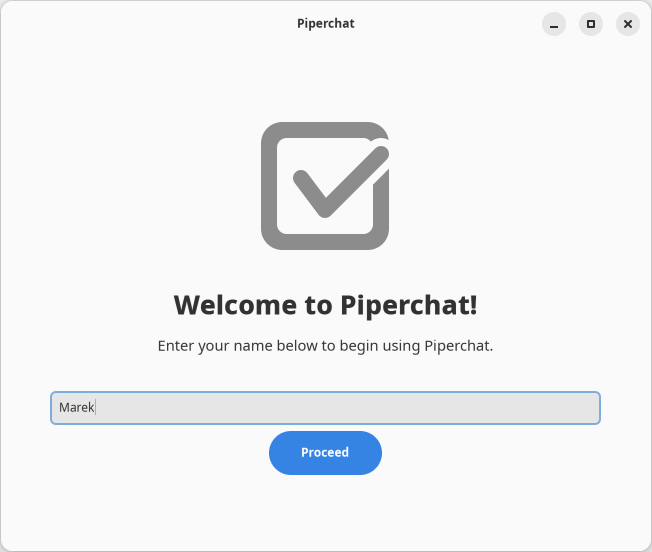
\includegraphics[width=.6\textwidth]{img/gui/screen_landing}
	\caption{Ekran lądowania}
\end{figure}

\subsubsection{Główny ekran aplikacji}

\begin{figure}[H]
	\centering
	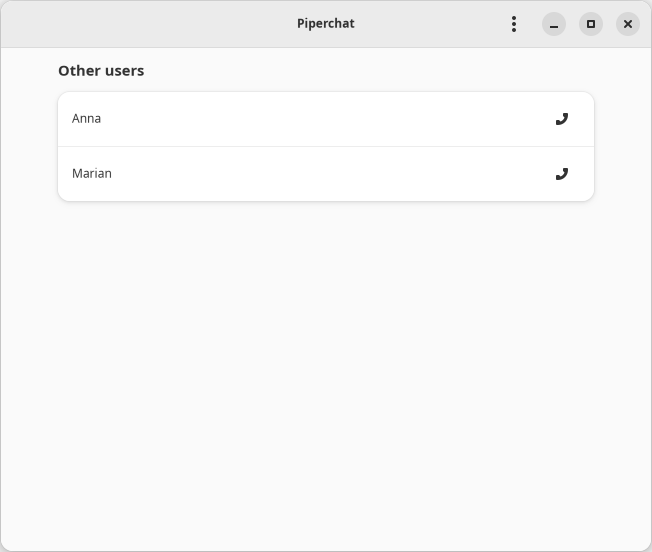
\includegraphics[width=.6\textwidth]{img/gui/screen_main}
	\caption{Główny ekran aplikacji}
\end{figure}

\subsubsection{Dialog wysłania połączenia}

\begin{figure}[H]
	\centering
	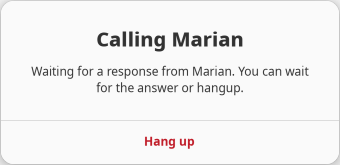
\includegraphics[width=.6\textwidth]{img/gui/screen_call_start}
	\caption{Dialog wysłania połączenia}
\end{figure}

\subsubsection{Dialog otrzymania połączenia}

\begin{figure}[H]
	\centering
	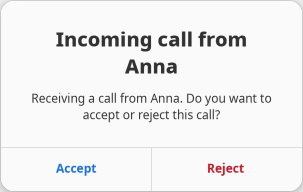
\includegraphics[width=.6\textwidth]{img/gui/screen_call_recv}
	\caption{Dialog otrzymania połączenia}
\end{figure}

\subsubsection{Dialog odrzucenia połączenia przez odbiorcę}

\begin{figure}[H]
	\centering
	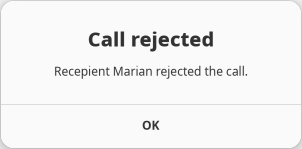
\includegraphics[width=.6\textwidth]{img/gui/screen_recepient_reject}
	\caption{Dialog odrzucenia połączenia przez odbiorcę}
\end{figure}

\subsubsection{Dialog porzucenia połączenia przez nadawcę}

\begin{figure}[H]
	\centering
	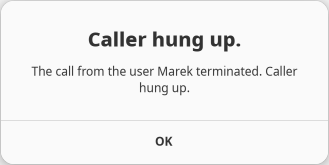
\includegraphics[width=.6\textwidth]{img/gui/screen_caller_hungup}
	\caption{Dialog porzucenia połączenia przez nadawcę}
\end{figure}
